\section{Time-reversal method}
\label{sec:pureshift__timerev}

This section focuses on the time-reversal element briefly introduced in \cref{subsec:pureshift__elements}: the aim is to determine whether a pure shift method based on this can have better performance than PSYCHE.
Before that, I will first provide a more detailed theoretical analysis of it.
The time-reversal element consists of just a single hard pulse with a flip angle $\beta$, and we first analyse its potential use as a JRE (instead of a PSE), using \cref{eq:ipm_beta_evolution,eq:ialpha_beta_evolution,eq:ibeta_beta_evolution}.

Recall that an ideal JRE should invert passive spins only, not active spins: thus, we seek a transformation of the form $I_{1+}I_{2\alpha} \to I_{1+}I_{2\beta}$.
However, the hard pulse does this:
\begin{equation}
    \label{eq:beta_pulse_not_jre}
    I_{1+}I_{2\alpha} \to
    {\underbrace{c^2s^2 I_{1+}I_{2\beta}}_{\text{term 1}}}
    + {\underbrace{c^4 I_{1+}I_{2\alpha}}_{\text{term 2}}}
    - {\underbrace{\frac{S^2}{4}I_{1\alpha}I_{2+} + \frac{S^2}{4}I_{1\beta}I_{2+}}_{\text{terms 3 and 4}}},
\end{equation}
where (as before) $S = \sin\beta$, $s = \sin(\beta/2)$, and $c = \cos(\beta/2)$.
As in the analysis for PSYCHE (\cref{subsec:pureshift__psyche_analysis}), term 1 here represents the desired signal; term 2 recoupling artefacts; and terms 3 and 4 COSY-type artefacts arising from coherence transfer.
Terms with difference coherence orders have been neglected as they can be removed using CTP gradients.\footnote{In the original work\autocite{Sorensen1985JACS} which predated widespread use of field gradients, other terms were removed through phase cycling, which is essentially equivalent.}
Unlike in the PSYCHE analysis, however, we have not neglected any other terms of smaller order in $s$.

Since the desired and undesired terms have different coefficients, it is possible to \textit{fully cancel out the recoupling artefacts} by recording (in this case) two different spectra with different values of $\beta$ and performing an appropriate linear combination:
\begin{align}
    I_{1+}I_{2\alpha} &\xrightarrow{\beta = \ang{0}} I_{1+}I_{2\alpha} \label{eq:timereversal_twospin_0} \\
    I_{1+}I_{2\alpha} &\xrightarrow{\beta = \ang{90}} \frac{1}{4}I_{1+}I_{2\beta} + \frac{1}{4}I_{1+}I_{2\alpha} - \frac{1}{4}I_{1\alpha}I_{2+} + \frac{1}{4}I_{1\beta}I_{2+} \label{eq:timereversal_twospin_90}
\end{align}
If we take \cref{eq:timereversal_twospin_90} minus $1/4$ of \cref{eq:timereversal_twospin_0}, the recoupling artefacts (arising from the $I_{1+}I_{2\alpha}$ term) are fully removed.
In general, for an $N$-spin system, there are several different `types' of recoupling artefacts where different numbers of passive spins (between 1 and $N - 1$) are not inverted.
Each of these pathways will have different coefficients, as each spin that is flipped contributes $s^2$, whereas each spin that is not flipped contributes $c^2$.
Suppressing all of these requires the acquisition and summation of $N$ spectra with different flip angles and appropriate weights.

Before we go on further, notice even in the two-spin system that the COSY-type artefacts are \textit{not} suppressed!
In the original work\autocite{Sorensen1985JACS}, this time-reversal element was used in the middle of the $t_1$ period in a NOESY experiment.
The coherence transfer peaks were not deemed to be problematic in this context: they gave rise to artefacts which had $F_1$ frequencies of $(\Omega_1 + \Omega_2)/2$, but different phase properties to genuine crosspeaks, allowing them to be easily identified.
Of course, these artefacts are not acceptable in an actual pure shift spectrum.

To remove these peaks, I adopted the strategy first reported by Thrippleton \textit{et al.} for suppression of COSY-type transfer pathways in 2DJ spectra.\autocite{Thrippleton2005JMR}
In a 2DJ experiment, the central \ang{180} pulse should in principle not cause coherence transfers between different spins; however, in strongly coupled systems this can happen.
The solution was to bracket the \ang{180} pulse, as well as half of the $t_1$ period, with a pair of opposing chirps and gradients.
The same idea was later used in the TSE-PSYCHE experiment\autocite{Foroozandeh2015CC} to (further) suppress strong coupling responses in the parent PSYCHE experiment.
This works because the unwanted CTPs have coherences on different spins during each of the two chirps; consequently, the coherences are inverted at different times by the chirp pulses, and are ultimately dephased by gradients.
The resulting time-reversal experiment was thus simply the same as the parent TSE-PSYCHE experiment, except that the central PSYCHE element was replaced by a $\beta$ hard pulse (\cref{fig:timereversal_pulseq}).

\begin{figure}[htb]
    \centering
    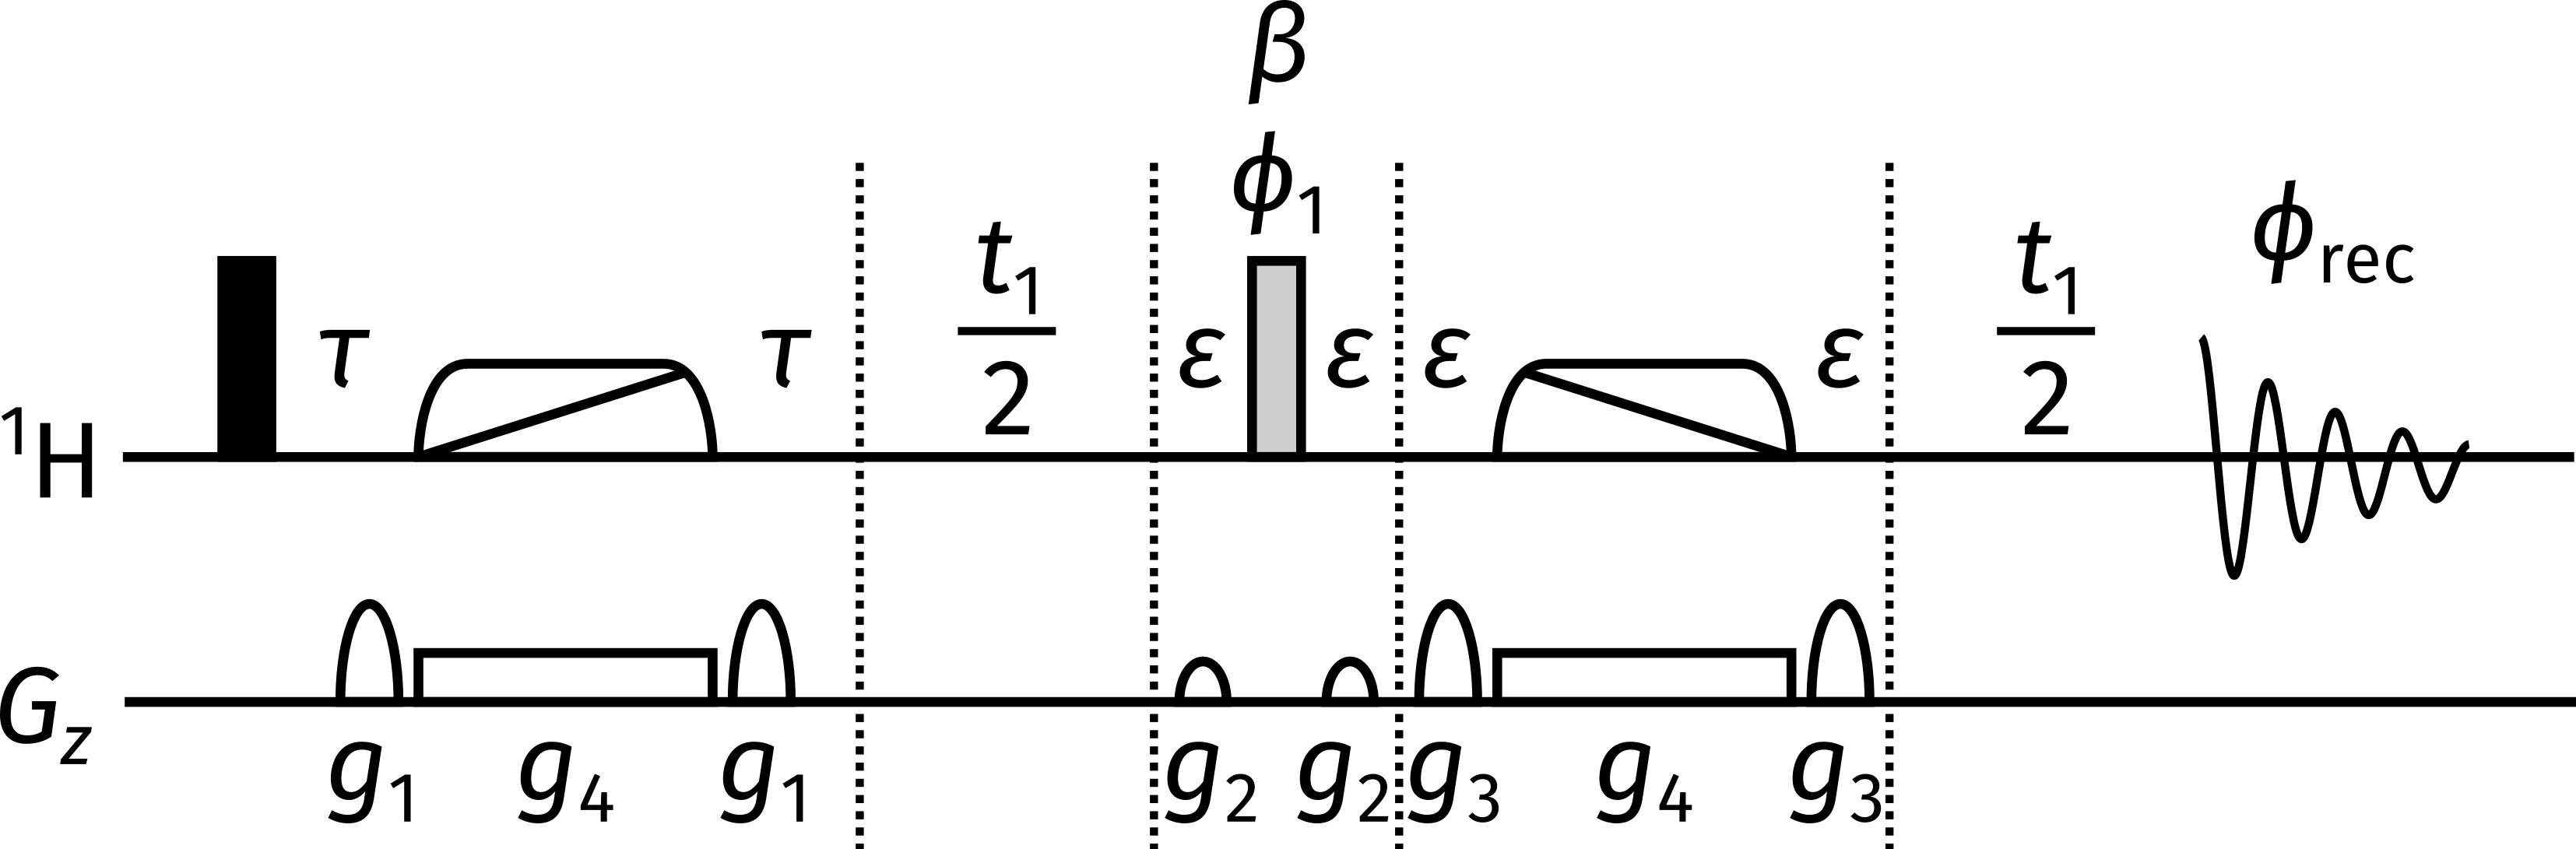
\includegraphics[]{pp/pureshift/timereversal.png}
    \caption[Time-reversal pure shift pulse sequence]{
        Time-reversal pure shift pulse sequence.
        The flip angle $\beta$ is varied as described in \cref{eq:timereversal_pse_angles}.
        Pulse phases are: $\phi_1 = (x, y, -x, -y)$; $\phi_\text{rec} = (x, -x, x, -x)$.
        The delay $\tau$ is set to $1/(4 \cdot T_\text{chunk})$, and allows for J-coupling to be refocused in the middle of the chunk.
        Gradient amplitudes are $(g_1, g_2, g_3, g_4) = (35\%, 49\%, 77\%, 1\%)$ (note that, in principle, $g_4$ should be calibrated according to the bandwidth of the chirp used).
    }
    \label{fig:timereversal_pulseq}
\end{figure}

In such a sequence, the JRE is in fact not only the $\beta$ pulse itself but also the second chirp (which effectively acts as a \ang{180} pulse).
So, the $\beta$ pulse here fulfils the role of a PSE, not a JRE: this means that different flip angles and weights must be chosen.
As before, for a system containing $N$ mutually coupled spins, $N$ different experiments must be acquired using the following flip angles $\beta_j$ and summed with the corresponding weights $W_j$ ($j = 1, 2, \ldots, N$):
\begin{align}
    \beta_j &= \frac{j\pi}{N} \label{eq:timereversal_pse_angles} \\
    W_j &= \frac{N}{8}\cdot \frac{(-1)^j}{\sin^2(\beta_j/2)} \label{eq:timereversal_pse_weights}.
\end{align}
For the sake of completeness, the values of $\beta$ and $W$ for a JRE are given here as well:
\begin{align}
    \beta_k &= \frac{k\pi}{N} \label{eq:timereversal_jre_angles} \\
    W_k &= \frac{N}{8}\cdot \frac{(-1)^{k + N}}{\cos^2(\beta_j/2)} \label{eq:timereversal_jre_weights}
\end{align}
for $k = 0, 1, \ldots, N-1$.
The derivation of these expressions is discussed more thoroughly in a paper by Griesinger et al.\autocite{Griesinger1986JCP}
In the context of this specific paper, note that the weights for the PSE correspond to that used for the ECOSY experiment, and the weights for the JRE correspond to that used for the complementary ECOSY experiment.

In practice, $N = 5$ is likely to cover most realistic spin systems.
Explicitly evaluating \cref{eq:timereversal_pse_angles,eq:timereversal_pse_weights} yields $\beta = \{\ang{36}, \ang{72}, \ang{108}, \ang{144}, \ang{180}\}$ and $W = \{−6.545,1.809,−0.955,0.691,−0.625\}$.
\Cref{fig:timereversal_insets} shows insets of the five subspectra acquired with the above values of $\beta$ and scaled by their respective weights $W$.
The weighted sum (i.e.\ the pure shift spectrum) was phased, and the resulting phase correction values were propagated back to the individual subspectra.

\begin{figure}[htb]
    \centering
    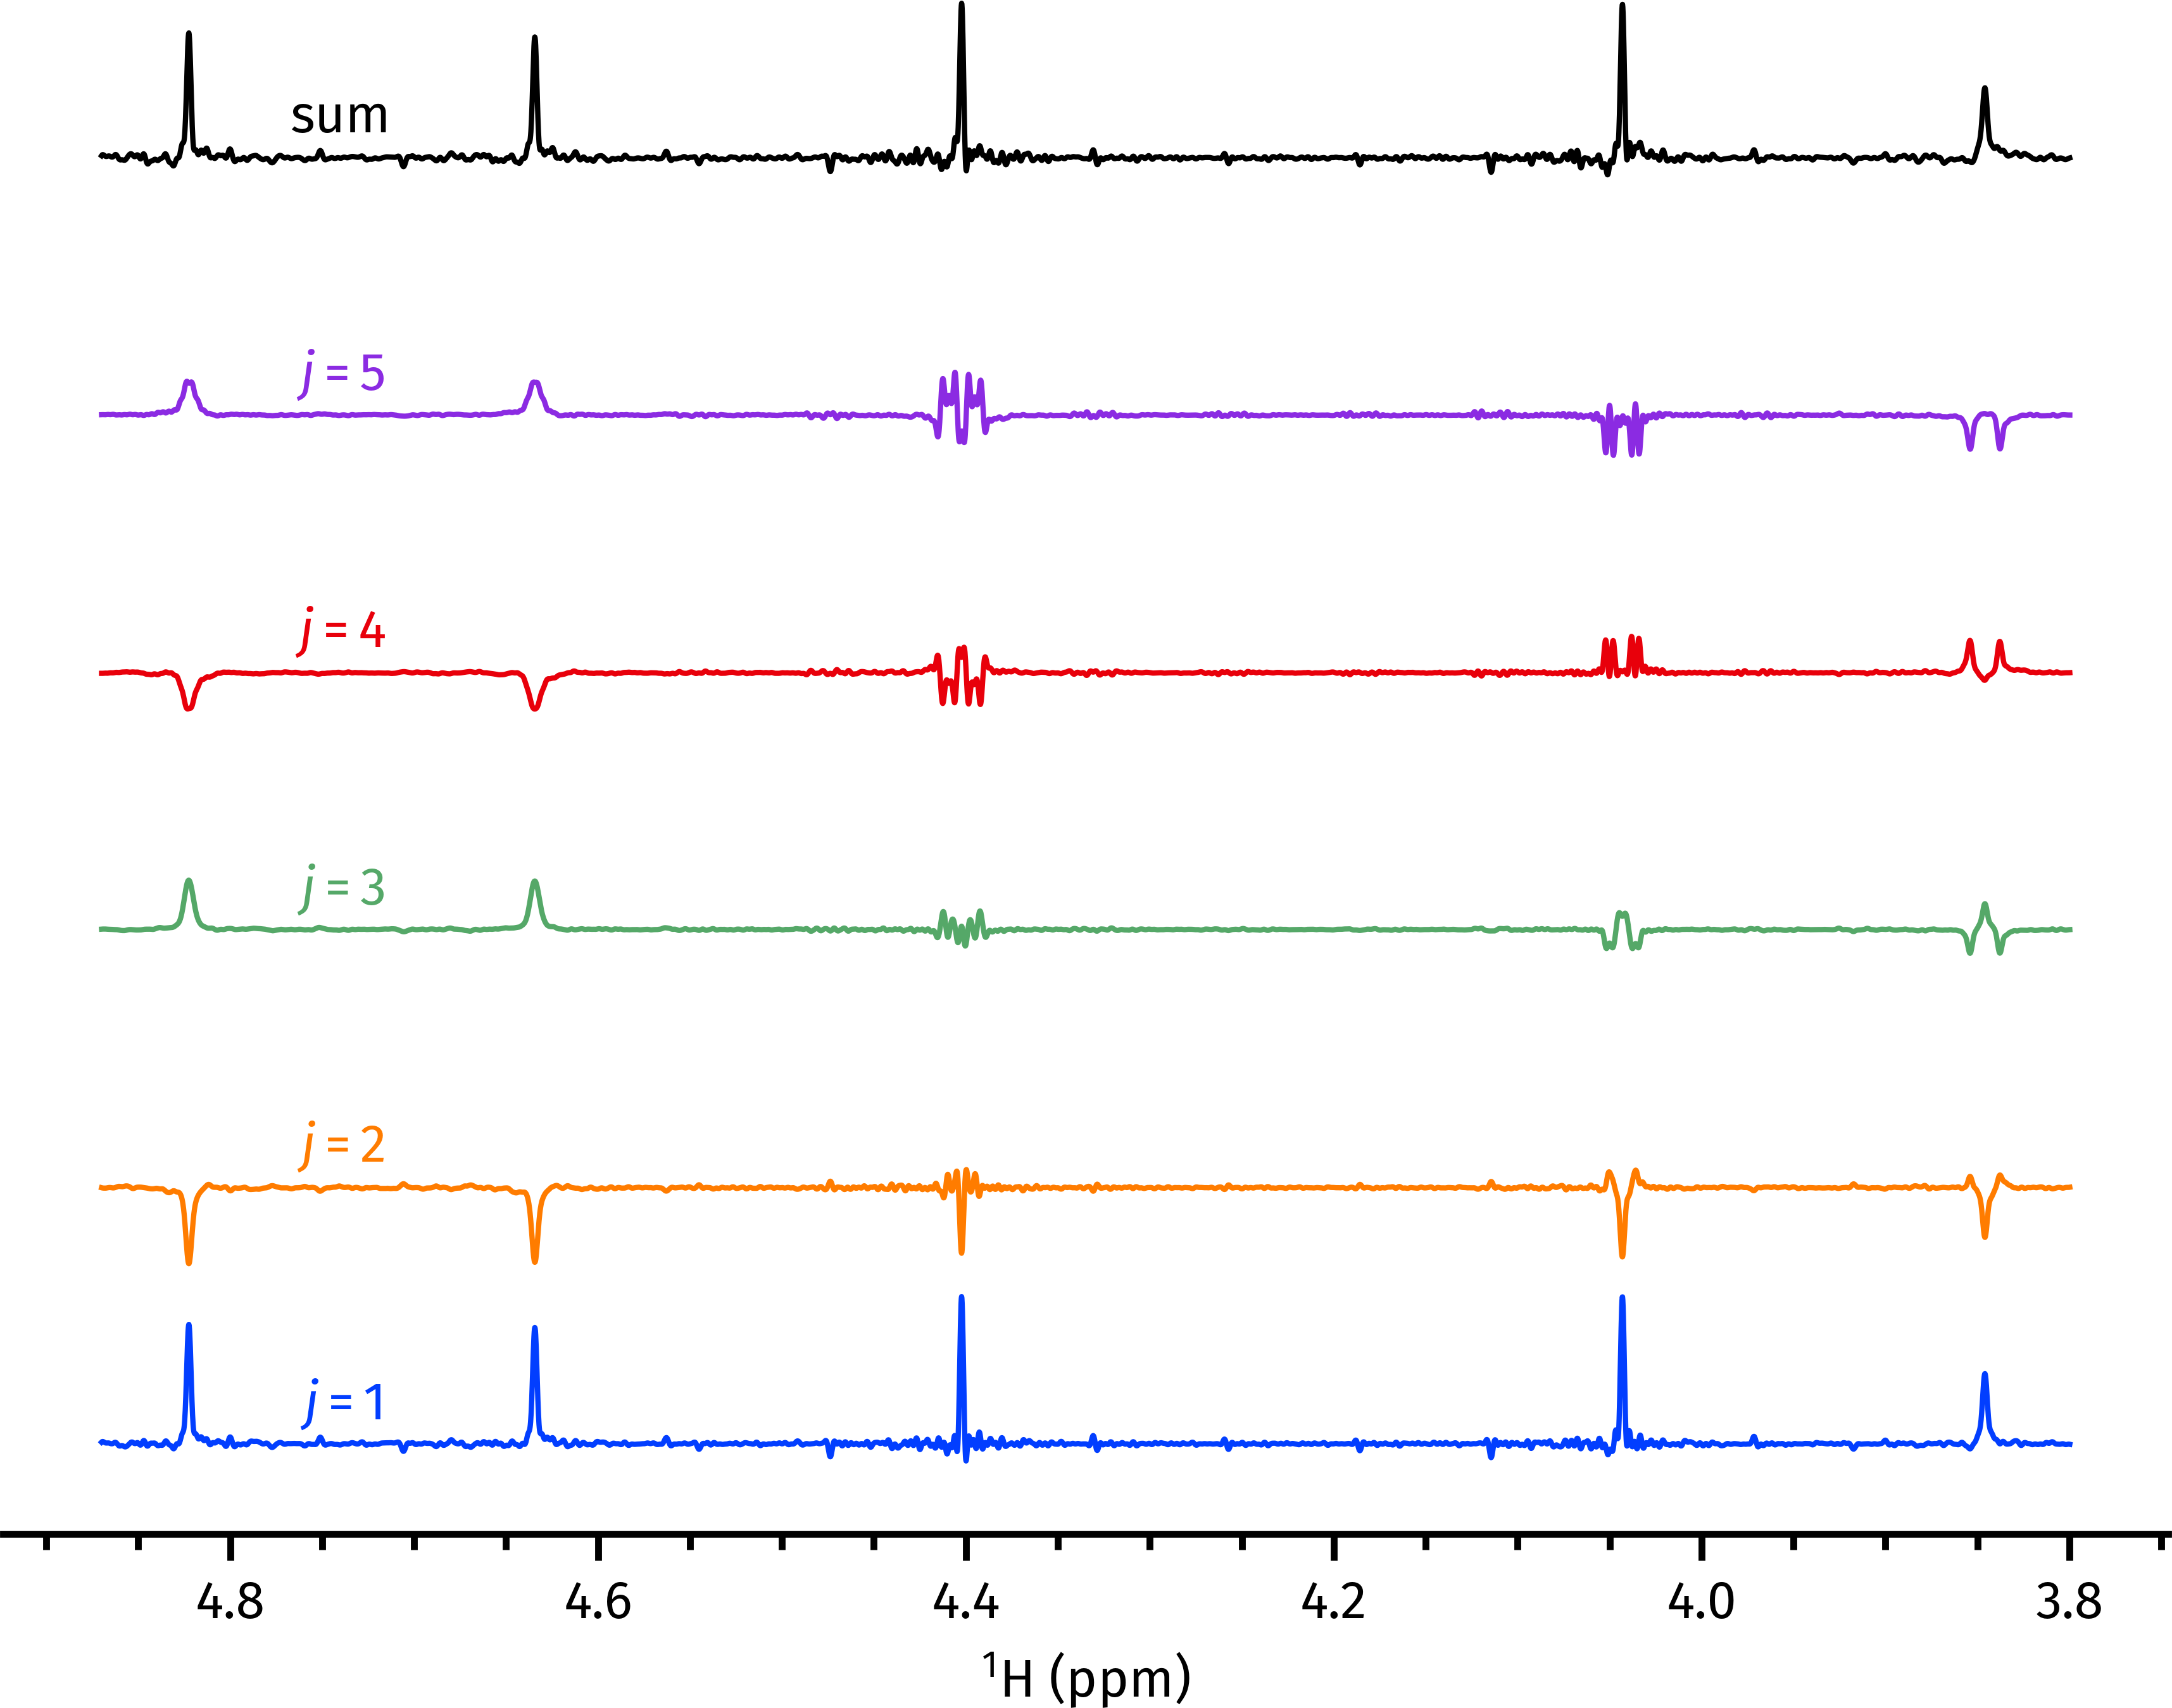
\includegraphics[]{pureshift/timereversal_insets.png}
    \caption[Insets of time-reversal spectra]{
        Insets of weighted time-reversal subspectra (with $j = 1$ through 5), as well as their sum (the pure shift spectrum).
        \datacode{7A-201020}
    }
    \label{fig:timereversal_insets}
\end{figure}

Although the experiment seems to work, in that the weighted sum \textit{is} indeed a pure shift spectrum, the fact that it is obtained through summation of $N$ different experiments brings some immediate drawbacks.
Firstly, the minimum duration of the experiment is lengthened by a factor of $N$: this is essentially the same as an $N$-step phase cycle.
However, and perhaps more importantly in the context of \textit{pure shift} NMR, the artefacts surrounding the main peaks are not perfectly cancelled through the process of summation.
As a result, random distortions are observed around the desired peaks in the pure shift spectrum: this is noticeable in the \SI{4.04}{ppm} peak in \cref{fig:timereversal_insets}, and is even worse for more intense signals.

In terms of sensitivity, the time-reversal spectrum is not particularly exceptional, either.
Each of the five subspectra above were acquired with 2 scans; when compared against a typical TSE-PSYCHE experiment acquired with only 4 scans (i.e.\ 40\% of the experiment duration), the TSE-PSYCHE experiment had comparable or perhaps even slightly better SNR (\cref{fig:timereversal_sensitivity}).
The likely reason for this is because in the time-reversal experiment, signal is actually being \textit{cancelled out} through the process of summation, as is quite clearly shown in \cref{fig:timereversal_insets}.
In principle, the sensitivity of the time-reversal experiment could be optimised by acquiring the more heavily weighted spectra with more scans.
However, I consider this unlikely to make a substantial difference to the conclusions drawn here.
The idea of re-optimising the weights to better suppress artefacts was also briefly considered.
However, given that \cref{eq:timereversal_pse_weights} already yields \textit{theoretically} complete suppression, it was deemed unlikely that anything substantially better could be obtained, considering that the artefacts arise from the summation process itself and are likely to appear regardless of what weights are chosen.
Performing such an optimisation would also require a pure shift spectrum to have been acquired beforehand (for comparison), thus defeating the purpose of optimising the weights anyway.

\begin{figure}[htb]
    \centering
    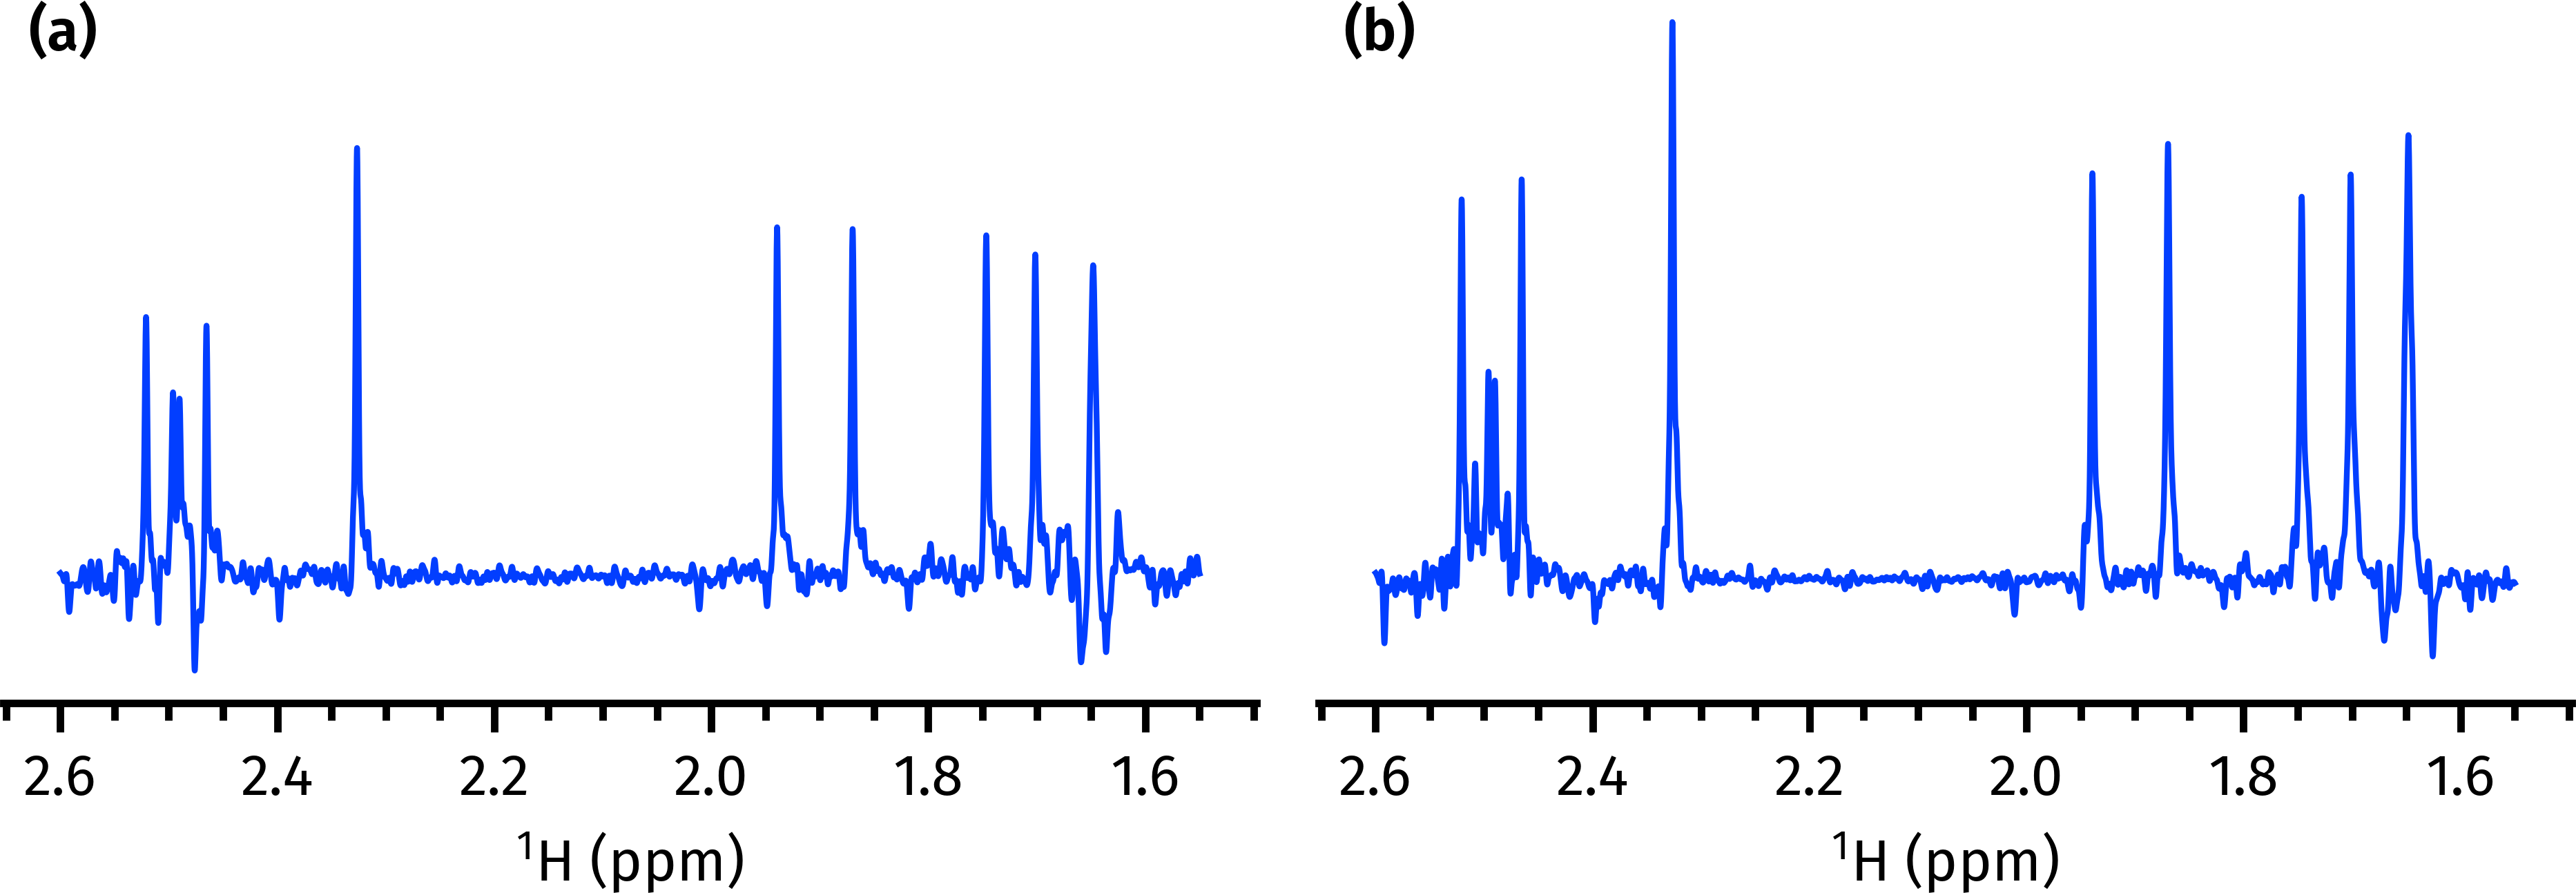
\includegraphics[]{pureshift/timereversal_sensitivity.png}
    {\phantomsubcaption\label{fig:timereversal_sensitivity_tr}}
    {\phantomsubcaption\label{fig:timereversal_sensitivity_tsepsyche}}
    \caption[Comparison of time-reversal and TSE-PSYCHE sensitivity]{
        Comparison of time-reversal and TSE-PSYCHE sensitivity.
        \textbf{(\subref{fig:timereversal_sensitivity_tr})} Time-reversal pure shift spectrum (the same as the sum in \cref{fig:timereversal_insets}) acquired with 2 scans for each subspectrum.
        \textbf{(\subref{fig:timereversal_sensitivity_tsepsyche})} TSE-PSYCHE (double saltire, flip angle \ang{15}) acquired with 4 scans.
        The spectra have been scaled so that their noise levels are similar: the signal intensity is comparable, or perhaps slightly better in the TSE-PSYCHE.
        \datacode{7A-201020}
    }
    \label{fig:timereversal_sensitivity}
\end{figure}

Interestingly, \cref{fig:timereversal_insets} suggests that the $j = 1$ spectrum \textit{on its own} already provides as good a result as the summed pure shift spectrum.
This is not surprising, as the use of a hard pulse as the PSE yields a conceptually very similar result to PSYCHE in that the signal to artefact ratio depends on $\tan^2(\beta/2)$ (of course, the COSY-type artefacts must still be suppressed through the TSE scheme).
This suggests that even without summation of multiple subspectra, the TSE time-reversal pulse sequence in \cref{fig:timereversal_pulseq} is a viable pure shift experiment---albeit one which does not have any significant advantage over PSYCHE.
